\documentclass[10pt,a4paper]{article}

\usepackage[top=1.8cm, bottom=2.0cm, left=1.8cm, right=1.8cm]{geometry}
\usepackage[utf8]{inputenc}
\DeclareUnicodeCharacter{20B9}{INR~}
\usepackage[T1]{fontenc}
\usepackage{helvet}
\renewcommand{\familydefault}{\sfdefault}
\usepackage{amsmath,amssymb}
\usepackage{xcolor}
\usepackage{booktabs}
\usepackage{tabularx}
\usepackage{colortbl}
\usepackage{tikz}
\usetikzlibrary{shapes.geometric, arrows.meta, positioning, fit, backgrounds, calc}
\usepackage{fancyhdr}
\usepackage{titlesec}
\usepackage{tcolorbox}
\tcbuselibrary{skins,breakable}
\usepackage{enumitem}
\usepackage{hyperref}

% Color Palette - Deep Slate & Modern Indigo / Emerald
\definecolor{primary}{HTML}{0F172A}       % Deep Slate 900
\definecolor{secondary}{HTML}{1E293B}     % Slate 800
\definecolor{accent}{HTML}{0284C7}        % Sky Blue 600
\definecolor{emerald}{HTML}{059669}       % Emerald 600
\definecolor{warning}{HTML}{D97706}       % Amber 600
\definecolor{lightbg}{HTML}{F8FAFC}       % Slate 50
\definecolor{bordercolor}{HTML}{E2E8F0}   % Slate 200
\definecolor{tableheader}{HTML}{1E293B}
\definecolor{tablerowalt}{HTML}{F1F5F9}

% Hyperref Setup
\hypersetup{
    colorlinks=true,
    linkcolor=accent,
    urlcolor=accent,
    citecolor=emerald,
    pdftitle={Kultura AI - Turnkey Private AI Infrastructure & Developer Operating Platform},
    pdfauthor={Kultura Founding Team}
}

% Header & Footer
\pagestyle{fancy}
\fancyhf{}
\fancyhead[L]{\textcolor{secondary}{\textbf{Kultura AI} \textbar\ Turnkey Private AI Infrastructure}}
\fancyhead[R]{\textcolor{secondary}{\footnotesize YC-Style Pitch \& Technical Blueprint}}
\fancyfoot[L]{\textcolor{gray}{\footnotesize Confidential \textbar\ Internal Founding Team \& Investor Review}}
\fancyfoot[R]{\textcolor{secondary}{\thepage}}
\renewcommand{\headrulewidth}{0.4pt}
\renewcommand{\footrulewidth}{0.4pt}

% Section Formatting
\titleformat{\section}{\large\bfseries\color{primary}}{\thesection.}{0.5em}{}[\titlerule]
\titleformat{\subsection}{\normalsize\bfseries\color{secondary}}{\thesubsection}{0.5em}{}
\titlespacing*{\section}{0pt}{12pt}{6pt}
\titlespacing*{\subsection}{0pt}{8pt}{4pt}

% Custom Callout Boxes
\newtcolorbox{pitchbox}[1][]{
    enhanced,
    colback=lightbg,
    colframe=accent,
    arc=4mm,
    boxrule=1pt,
    title=\textbf{#1},
    coltitle=white,
    colbacktitle=accent,
    fonttitle=\bfseries,
    attach boxed title to top left={xshift=4mm, yshift=-2mm},
    boxed title style={size=small, colframe=accent},
    top=8pt, bottom=8pt, left=10pt, right=10pt
}

\newtcolorbox{metricbox}[1][]{
    enhanced,
    colback=lightbg,
    colframe=emerald,
    arc=3mm,
    boxrule=0.8pt,
    top=6pt, bottom=6pt, left=8pt, right=8pt
}

\begin{document}

% Title Header
\begin{center}
    {\Huge \textbf{\textcolor{primary}{KULTURA AI}}}\\[4pt]
    {\large \textbf{\textcolor{secondary}{Turnkey Private AI Infrastructure \& Developer Operating Platform}}}\\[3pt]
    {\footnotesize \textcolor{gray}{YC-Style Pitch Deck, Production Engineering Blueprint \& Commercial Financial Model \textbar\ November 2026}}
\end{center}
\vspace{-4pt}
\hrule height 1.2pt
\vspace{8pt}

% Executive Pitch Callout
\begin{pitchbox}[EXECUTIVE PITCH \& CORE VALUE PROPOSITION]
\textbf{The One-Line Pitch:} \textit{Kultura is a self-hosted private AI platform that gives companies an internal ChatGPT for employees and a private Copilot endpoint for developers---deployed in their own AWS VPC in 15 minutes, cutting AI costs by 45\% while guaranteeing zero data leaks.}

\vspace{4pt}
\textbf{The 60-Second Problem \& Solution Thesis:}
Mid-market enterprises with 50 to 500 staff face a compounding crisis: developers use GitHub Copilot while non-tech staff use ChatGPT. For a 200-person firm, this burns \textbf{\$4,400/month (\$52,800/year)} in disconnected SaaS seats. Far worse: proprietary client code, financial records, and employee data continuously leak into public cloud models, violating client Master Services Agreements (MSAs). 

Kultura deploys a containerized platform inside the client's AWS VPC or on-premise GPU. It gives staff a private ChatGPT connected to Google Drive, and gives developers an OpenAI-compatible Copilot endpoint in VS Code powered by \textbf{Qwen-2.5-Coder-32B} (delivering 90\% of Claude 3.5 Sonnet's coding intelligence). With 3-tier RBAC and local PII scrubbing, Kultura slashes annual spend by 45\%--62\% with mathematical data privacy.
\end{pitchbox}

\section{System Architecture \& Dual Ingress Interfaces}

Kultura deploys as a containerized appliance inside the customer's security boundary. It exposes two specialized front-doors:

\vspace{4pt}
\begin{center}
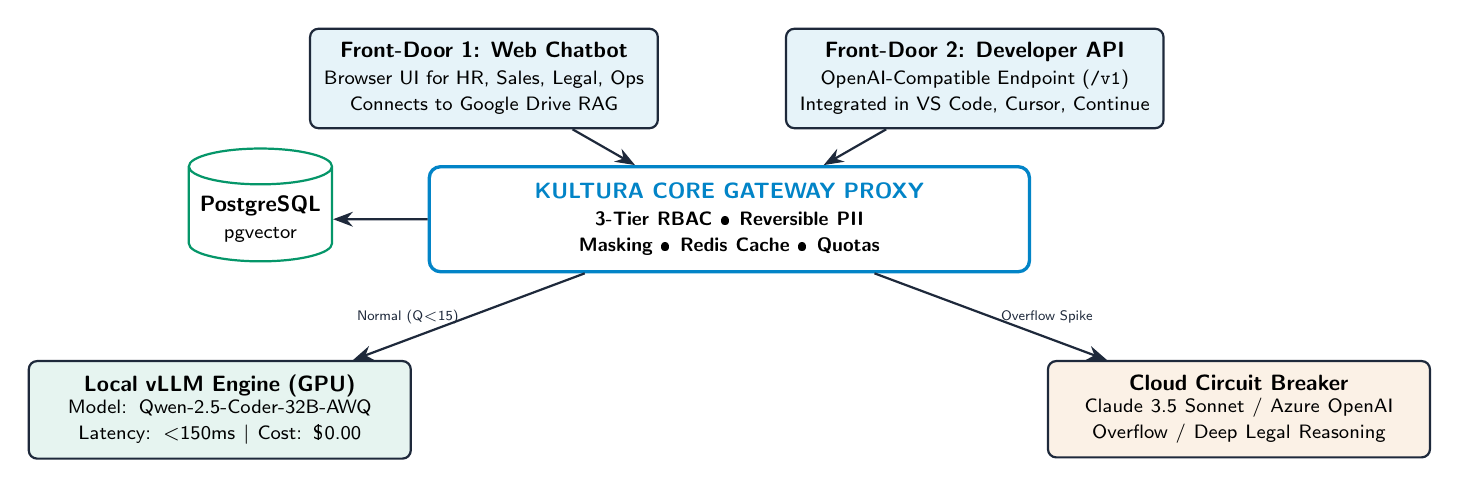
\begin{tikzpicture}[
    node distance=0.85cm and 1.2cm,
    box/.style={rectangle, draw=secondary, fill=lightbg, rounded corners=3pt, thick, align=center, font=\footnotesize, inner sep=5pt},
    headerbox/.style={rectangle, draw=primary, fill=primary, text=white, rounded corners=3pt, thick, align=center, font=\bfseries\footnotesize, inner sep=4pt},
    gateway/.style={rectangle, draw=accent, fill=white, rounded corners=4pt, very thick, align=center, font=\footnotesize\bfseries, inner sep=6pt},
    storage/.style={cylinder, shape border rotate=90, draw=emerald, fill=white, aspect=0.25, thick, align=center, font=\footnotesize, inner sep=4pt},
    arrow/.style={-{Stealth[length=2.5mm]}, thick, color=secondary}
]

% Dual Ingress
\node[box, fill=accent!10] (FD1) {\textbf{Front-Door 1: Web Chatbot}\\\scriptsize Browser UI for HR, Sales, Legal, Ops\\\scriptsize Connects to Google Drive RAG};
\node[box, fill=accent!10, right=1.6cm of FD1] (FD2) {\textbf{Front-Door 2: Developer API}\\\scriptsize OpenAI-Compatible Endpoint (\texttt{/v1})\\\scriptsize Integrated in VS Code, Cursor, Continue};

% Core Gateway
\node[gateway, below=1.1cm of $(FD1)!0.5!(FD2)$, text width=7.2cm] (GW) {
    \textcolor{accent}{KULTURA CORE GATEWAY PROXY}\\
    \scriptsize 3-Tier RBAC \textbullet\ Reversible PII Masking \textbullet\ Redis Cache \textbullet\ Quotas
};

% Storage
\node[storage, left=1.2cm of GW] (PG) {\textbf{PostgreSQL}\\\scriptsize pgvector};

% Execution Layer
\node[box, fill=emerald!10, below left=1.1cm and 0.2cm of GW, text width=4.5cm] (LocalGPU) {
    \textbf{Local vLLM Engine (GPU)}\\\scriptsize Model: Qwen-2.5-Coder-32B-AWQ\\\scriptsize Latency: $<$150ms \textbar\ Cost: \$0.00
};

\node[box, fill=warning!10, below right=1.1cm and 0.2cm of GW, text width=4.5cm] (CloudAPI) {
    \textbf{Cloud Circuit Breaker}\\\scriptsize Claude 3.5 Sonnet / Azure OpenAI\\\scriptsize Overflow / Deep Legal Reasoning
};

% Connectors
\draw[arrow] (FD1) -- (GW);
\draw[arrow] (FD2) -- (GW);
\draw[arrow] (GW) -- (PG);
\draw[arrow] (GW) -- node[left, font=\tiny]{Normal (Q$<$15)} (LocalGPU);
\draw[arrow] (GW) -- node[right, font=\tiny]{Overflow Spike} (CloudAPI);

\end{tikzpicture}
\end{center}

\vspace{-4pt}
\begin{itemize}[leftmargin=12pt, itemsep=1pt]
    \item \textbf{Front-Door 1 (Internal Staff Chat):} Browser UI at \texttt{ai.internal.company.com} synced with Google Drive.
    \item \textbf{Front-Door 2 (Developer Endpoint):} Drop-in OpenAI-compatible API at \texttt{ai.internal.company.com/v1}.
\end{itemize}

\section{Model Selection: Researched Open-Weights Benchmarks}

To achieve \textbf{88\%--92\% of Claude 3.5 Sonnet's coding power} without massive enterprise GPU clusters, Kultura utilizes 4-bit AWQ quantized architectures fitting into single 24GB GPUs:

\vspace{4pt}
\begin{tabularx}{\textwidth}{l p{4.2cm} l X}
\toprule
\rowcolor{tableheader}
\textcolor{white}{\textbf{Workload Role}} & \textcolor{white}{\textbf{Selected Model}} & \textcolor{white}{\textbf{VRAM / Quant}} & \textcolor{white}{\textbf{Benchmark Justification \& Intelligence}} \\
\midrule
\textbf{Heavy Multi-File Coding} & \texttt{Qwen2.5-Coder-32B-Instruct} & AWQ (20--22GB) & \textbf{Matches GPT-4o (92.7\% HumanEval)}; 88--92\% Claude 3.5; 128k context; runs on 1x 24GB GPU. \\
\rowcolor{tablerowalt}
\textbf{Fast Autocomplete (IDE)} & \texttt{Qwen2.5-Coder-7B-Instruct} & AWQ ($\sim$5GB) & Sub-60ms time-to-first-token; low latency streaming during active keystroke typing. \\
\textbf{RAG Document Embeddings} & \texttt{nomic-embed-text-v1.5} & FP16 ($\sim$1.2GB) & Outperforms OpenAI \texttt{text-embedding-3-small} on MTEB; runs 100\% free locally. \\
\rowcolor{tablerowalt}
\textbf{Cloud Fallback Safety} & Anthropic Claude 3.5 Sonnet & Cloud HTTPS & Used only when local GPU queue is saturated. PII is scrubbed before egress. \\
\bottomrule
\end{tabularx}

\section{AWS Cloud Infrastructure Specifications \& Monthly Bill}

Deployed inside the client's AWS account within an isolated VPC with private subnets:

\vspace{4pt}
\begin{tabularx}{\textwidth}{l X r r}
\toprule
\rowcolor{tableheader}
\textcolor{white}{\textbf{AWS Service}} & \textcolor{white}{\textbf{Exact Resource Configuration}} & \textcolor{white}{\textbf{On-Demand / Mo}} & \textcolor{white}{\textbf{1-Yr Savings Plan}} \\
\midrule
\textbf{EC2 GPU Host} & \textbf{\texttt{g5.xlarge}} (1x NVIDIA A10G 24GB VRAM, 4 vCPU, 16GB RAM) & \$734.38 & \$514.00 \\
\rowcolor{tablerowalt}
\textbf{Amazon RDS} & \texttt{db.t4g.medium} (2 vCPU, 4GB RAM, 50GB gp3 with \texttt{pgvector}) & \$52.00 & \$38.00 \\
\textbf{Load Balancer} & AWS Application Load Balancer (ALB with ACM SSL Certificate) & \$22.50 & \$22.50 \\
\rowcolor{tablerowalt}
\textbf{EBS gp3 Storage} & 150GB gp3 NVMe (OS, model checkpoints, docker layer cache) & \$12.00 & \$12.00 \\
\midrule
\textbf{TOTAL INFRASTRUCTURE} & \textbf{Full Production-Grade In-VPC Appliance} & \textbf{\$820.88 / mo} & \textbf{\$586.50 / mo} \\
\bottomrule
\end{tabularx}

\section{On-Premise Alternative: Zero Monthly Cloud GPU Bills}

For Indian IT services, software agencies, and FinTech NBFCs, Kultura can run on an \textbf{Office AI Workstation}:
\begin{itemize}[leftmargin=12pt, itemsep=1pt]
    \item \textbf{Hardware Specification:} 1x Tower Workstation with \textbf{1x NVIDIA RTX 4090 (24GB VRAM)} OR \textbf{2x RTX 3090 (48GB total)}, AMD Ryzen 9, 64GB DDR5 RAM, 2TB NVMe SSD.
    \item \textbf{One-Time Capital Expenditure:} \textbf{₹2,80,000 to ₹3,40,000 (\$3,500 to \$4,000)}.
    \item \textbf{Amortized Cost (36 Months):} \textbf{\$105 / month} + \$30/month electricity = \textbf{\$135 / month total infra bill}!
    \item \textbf{Financial Impact:} Eliminates the \$734/month AWS bill, saving an extra \textbf{\$8,100 (₹6.8 Lakhs) every year}.
\end{itemize}

\section{The 200-User Enterprise Financial Model: BEFORE vs. AFTER}

The complete financial comparison for a company with \textbf{200 employees} (100 Developers + 100 Non-Tech Staff):

\vspace{4pt}
\begin{tabularx}{\textwidth}{l X X X}
\toprule
\rowcolor{tableheader}
\textcolor{white}{\textbf{Cost Component}} & \textcolor{white}{\textbf{BEFORE: Commercial SaaS}} & \textcolor{white}{\textbf{AFTER: Kultura on AWS}} & \textcolor{white}{\textbf{AFTER: Kultura On-Prem}} \\
\midrule
\textbf{100 Developers} & 100x GitHub Copilot @ \$19 = \$1,900 & Included in platform & Included in platform \\
\rowcolor{tablerowalt}
\textbf{100 Non-Tech Staff} & 100x ChatGPT Team @ \$25 = \$2,500 & Included in platform & Included in platform \\
\textbf{Infrastructure Cost} & \$0 (Hosted by OpenAI/Microsoft) & AWS \texttt{g5.xlarge} + RDS = \$820/mo & 1x Server Amortization = \$135/mo \\
\rowcolor{tablerowalt}
\textbf{Cloud Fallback Tokens} & \$0 & \$250 / mo (Overflow API) & \$250 / mo (Overflow API) \\
\textbf{Kultura License Fee} & \$0 & \$1,299 / mo (Software fee) & \$1,299 / mo (Software fee) \\
\midrule
\textbf{TOTAL MONTHLY BILL} & \textbf{\$4,400 / month (₹3,70,000)} & \textbf{\$2,369 / month (₹1,99,000)} & \textbf{\$1,684 / month (₹1,41,000)} \\
\rowcolor{tablerowalt}
\textbf{TOTAL ANNUAL SPEND} & \textbf{\$52,800 / year (₹44.4 Lakhs)} & \textbf{\$28,428 / year (₹23.9 Lakhs)} & \textbf{\$20,208 / year (₹17.0 Lakhs)} \\
\midrule
\textbf{NET ANNUAL SAVINGS} & \textbf{BASELINE (Zero Savings)} & \textbf{SAVE \$24,372 / YR (46.2\%)} & \textbf{SAVE \$32,592 / YR (61.7\%)} \\
\rowcolor{tablerowalt}
\textbf{Data Privacy Level} & High Risk (Code sent to US cloud) & \textbf{100\% In-VPC (Zero Leaks)} & \textbf{100\% Air-Gapped (Zero Leaks)} \\
\bottomrule
\end{tabularx}

\section{Concurrency Reality: Can 1x GPU Handle 40--50 Developers?}

\begin{itemize}[leftmargin=12pt, itemsep=2pt]
    \item \textbf{Peak vs. Continuous Concurrency:} 50 active developers do not generate 50 parallel requests at the same millisecond. Keystroke autocomplete triggers generate an average of \textbf{2 to 5 concurrent in-flight calls}, peaking at 8 to 12.
    \item \textbf{vLLM Continuous Batching:} Unlike default sequential inference, vLLM batches parallel requests into a single GPU computation, delivering \textbf{180--240 tokens/second aggregate throughput} on an A10G.
    \item \textbf{Circuit Breaker Fail-Safe:} If the local GPU queue depth exceeds 15 requests, Kultura automatically scrubs PII and routes overflow prompts to cloud fallback APIs. Response latency remains sub-second without server crashes.
\end{itemize}

\section{What Needs to Be Built: Developer Action Plan}

\begin{enumerate}[leftmargin=14pt, itemsep=2pt]
    \item \textbf{Model Pod:} Dockerized vLLM running \texttt{Qwen/Qwen2.5-Coder-32B-Instruct-AWQ} on port 8000.
    \item \textbf{Core Proxy:} Node.js 22 LTS / Fastify reverse proxy handling \texttt{/v1/chat/completions} streaming.
    \item \textbf{DLP Masking Middleware:} High-speed regex/NER engine for Aadhaar, PAN, SSN, and API key tokenization.
    \item \textbf{3-Tier RBAC:} PostgreSQL schema for Admin, Team Lead, and Developer roles with spending quotas.
    \item \textbf{RAG Sync Worker:} Node.js cron syncing Google Drive/SharePoint every 15 minutes using incremental hashing.
    \item \textbf{Web UI:} Next.js 15, Tailwind, and Shadcn UI dark-mode chat and admin cockpit.
\end{enumerate}

\section{Client Proposal Script: The 14-Day Risk-Free Pilot}

\begin{pitchbox}[OUTREACH TEMPLATE FOR CTOS AND HEADS OF ENGINEERING]
\textbf{Subject:} Eliminating Copilot code leaks \& cutting your AI bill by 45\%

\vspace{3pt}
\textit{``Hi [First Name], if your developers use GitHub Copilot and your staff use ChatGPT, you're likely spending \$3,000--\$5,000/month across disconnected accounts while risking client NDA violations by sending proprietary code to public models. We built \textbf{Kultura}, a self-hosted AI platform deployed in your AWS VPC in 15 minutes. It gives your developers a private Copilot powered by Qwen-2.5-Coder-32B (matching 90\% of Claude 3.5 Sonnet's coding power) and an internal ChatGPT for Google Drive. Can I deploy a free 14-day parallel pilot in your staging VPC this Thursday? We'll demonstrate an instant 40\%+ cost reduction with zero data leaks.''}
\end{pitchbox}

\end{document}
